\documentclass{ximera}

\author{Anna Davis} \title{MTH 160 Homework 11} 

\begin{document}

\begin{abstract}

\end{abstract}
\maketitle
 \textit{Certificate due: 4/21/2021 at 11:59 p.m.}
 \section{Lecture 25}

\begin{problem}\label{prob:160hom10prob7}
Find the missing coordinate.  Round your answers to two decimal places.
\begin{image}
   
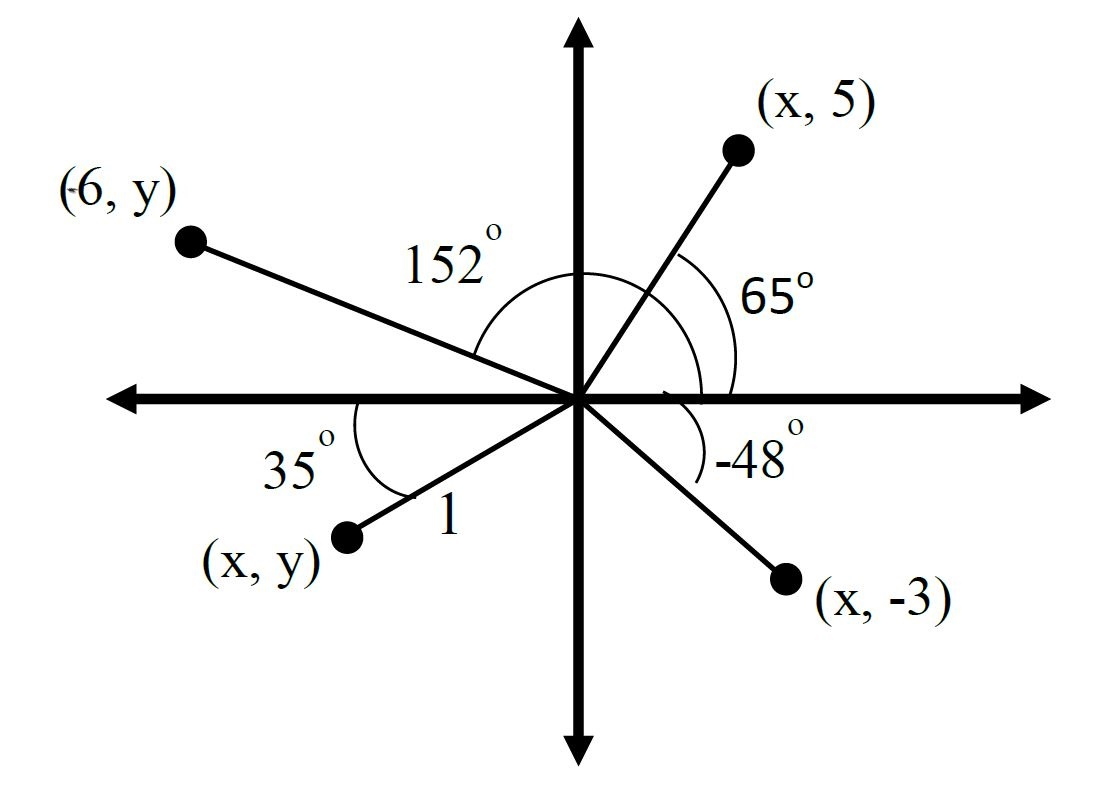
\includegraphics[height=1in]{160H10pic2.jpg}~
 
\end{image}

Quadrant I:
$$x=\answer[tolerance=0.01]{2.33}$$

Quadrant II:
$$y=\answer[tolerance=0.01]{3.19}$$

Quadrant III:
$$x=\answer{-0.82},\quad y=\answer{-0.57}$$

Quadrant IV:
$$x=\answer[tolerance=0.01]{2.7}$$
\end{problem}

\begin{problem}\label{prob:160hom10prob8}
Find $y$.  Round your answer to two decimal places.
 
 \begin{image}
   
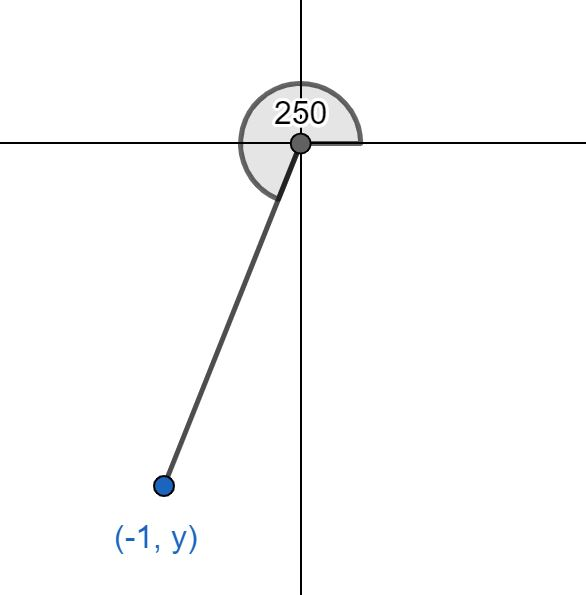
\includegraphics[height=1in]{160H10pic1.jpg}

\end{image}
$$y=\answer[tolerance=0.01]{-2.75}$$
\end{problem}

 
 
 
 
 
 
  \section{Lecture 26}
  \begin{problem}\label{prob:160hom11prob2}
  Find the amplitude and the period of the graph.
  \begin{image}
   
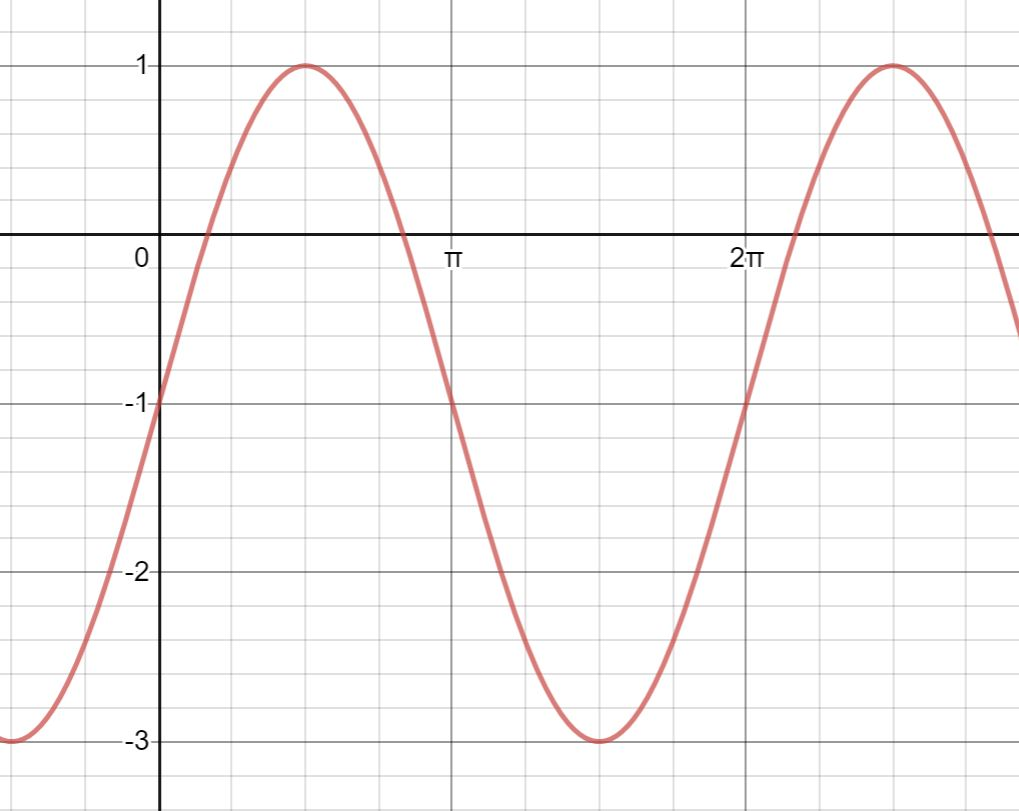
\includegraphics[height=1in]{160H11pic2.jpg}~
 
\end{image}
Amplitude: $\answer{2}$

Period: $\answer{2\pi}$
  \end{problem}
  
 \begin{problem}\label{prob:160hom11prob3}  
 The graph below has a slider that controls the value of $a$.  Use the slider to change the value of $a$ and find the period of each graph.
  \begin{center} 
\desmos{thhxefls5a}{800}{600} 
\end{center}
\begin{enumerate}
    \item Let $a=1$.  Period: $\answer{2\pi}$
    \item Let $a=2$.  Period: $\answer{\pi}$
    \item Let $a=3$.  Period: $\answer{\frac{2\pi}{3}}$
    \item Let $a=4$.  Period: $\answer{\pi/2}$
\end{enumerate}
In general, the period of $f(x)=\sin (ax)$ is $\answer{\frac{2\pi}{a}}$.
\end{problem}

\begin{problem}\label{prob:160hom11prob4}  
 The graph below has a slider that controls the value of $a$.  Use the slider to change the value of $a$ and find the period of each graph.
  \begin{center} 
\desmos{ow1opu7xy8}{800}{600} 
\end{center}
\begin{enumerate}
    \item Let $a=1$.  Period: $\answer{2\pi}$
    \item Let $a=0.5$.  Period: $\answer{4\pi}$
    \item Let $a=0.25$.  Period: $\answer{8\pi}$
    \item Let $a=0.75$.  Period: $\answer{\frac{8\pi}{3}}$
\end{enumerate}
In general, the period of $f(x)=\cos (ax)$ is $\answer{\frac{2\pi}{a}}$.
\end{problem}

\section{Lecture 27}

\begin{problem}\label{prob:160hom11prob5}  
 The graph below has a slider that controls the value of $a$. 
  \begin{center} 
\desmos{9fnipvn89y}{800}{600} 
\end{center}
Use the slider to experiment with the graphs and determine which of the following statements is true.
\begin{multipleChoice}  
\choice{$\cot\left(x+\frac{\pi}{2}\right)=\tan x$}  
\choice{$\cot x=-\tan x$}  
\choice{$\cot\left(x-\frac{\pi}{2}\right)=\tan x$}  
\choice[correct]{$\cot\left(x-\frac{\pi}{2}\right)=-\tan x$} 
\end{multipleChoice}  
\end{problem}  
  



\end{document} 